\subsection{Frame Stack Generation}
Although the geometry is three dimensional, the holographic printer works by virtually photographing two dimensional image sequences.  These sequences (or frames) are put together as stack, and fed to the  digital holographic printer.  Using a spatial light modulator, the printer invokes a pixel swapping algorithm that connects the various points in 2D space, adding relational z-depth cue information thus forming a three dimensional recording.\\

This process of creating an image stack is necessary to feed information to the printer, and is crucial in generating the overall scene design of the hologram viewed by the observer. As a result, we explore two image processing avenues using a set of 8-bit color images and a set of higher color depth images to compare aesthetic differences. 32-bit HDR images are of interest to investigate further in formats such as OpenEXR \cite{kainz2009technical}. However, due to the nature of creating an HDR image requires either bracketed capture from the imaging device, or the making of 32-bit images directly from the source, we opt for investigating this scenario in the next stage of the research. Additional challenges surfaced when researching the use of OpenEXR and the accessible toolbox of choice of software including Photoshop CC 2019, which at the time writing this, only supported exporting 16-bit OpenEXR files (half float).  ImageMagick, another tool of choice, a command line interface (CLI), also limited use of OpenEXR to 16-bit.\\

In addition to working with HDR images, working with linear colour space is to be considered throughout the pipeline until applying gamma correction for display purposes.  All monochromatic wavelengths are mapped to what is known as the ``spectral locus" of the CIE xy chromaticity diagram \cite{mansencal_thomas_2018_2647615} \cite{reinhard2010high}, familiar territory for holographers when working with colour, lasers, and optics.  Consideration will be given to testing the use of linear colour editing versus the common sRBG colour mode used traditionally with our partners holographic printer.  We believe the digital ``hard copy" nature of our hologram will benefit from looking beyond the sRGB color space.

\begin{figure}[H]
  \centering
  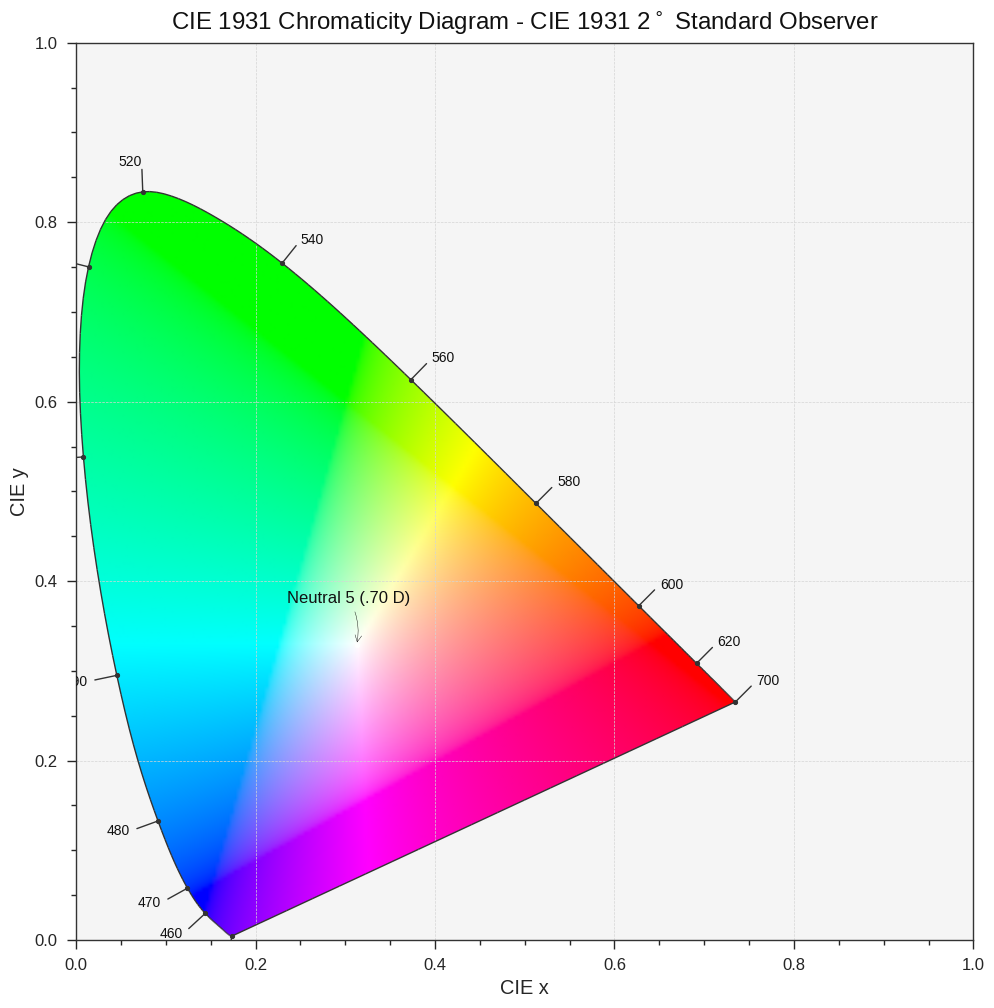
\includegraphics[width=\linewidth]{img/cie.png}
  \caption{CIE 1931 Chromaticity Diagram from \cite{mansencal_thomas_2018_2647615}}
  \Description{Spectral locus}
\end{figure}

Embedding an understanding of both linear space and gamma space into our workflow, could significantly change the very aesthetic of the images when viewed with color gamuts of digital displays, as such, should have an impact on the experience on the produced digital hologram.  One way to test these differences in our proposed pipeline is to test the making our image stack by incorporating the above stated factors in our production.

\\